\chapter{Leksička analiza}

\section{Uvod}
Cilj leksičkog analizatora je grupirati znakove u smislene cjeline --- lekseme. Primjerice, identifikatore i ključne riječi.
Time ćemo olakšati rad sintaksnom analizatoru i izgradnju samog sintaksnog analizatora tj. gramatike.

Leksički analizator čita izvorni kôd znak po znak, grupira znakove u lekseme, odbacuje bjeline, prikuplja podatke koje može prikupiti u tom trenutku (vrsta leksema, tip konstante), pronalazi eventualne pogreške i određuje mjesto u programu gdje je došlo do nje.

Leksički analizatori se realiziraju pomoću konačnih automata, a praksa je da se pravila zadaju regularnim izrazima.

\section{Implementacija}

Za implementaciju smo koristili alat jFlex koji na temelju zadanih pravila generira leksički analizator. jFlex je
alat za progamski jezik Javu tj. kôd analizatora koji generira je u Javi.

Razred koji generira i koji predstavlja leksički analizator u našem se slučaju zove \texttt{Lexer}. Prilikom
instanciranja razreda \texttt{Lexer}, konstruktor prima \texttt{InputStream} iz kojeg čita ulaznu datoteku (izvorni kôd),
objekt razreda \texttt{Table} u koji će puniti informacije o leksemima (tip leksema, tip konstante) i listu u koju će
redom dodavati lekseme (kako bi ih kasnije mogli prikazati u tablici korisničkog sučelja).

Leksemi su predstavljeni razredom \texttt{Token} koji nasljeđuje razred \texttt{java\_cup.runtime.Symbol} (objekte tog razreda
očekuje sintaksni analizator generiran CUP-om, o tome kasnije). 

Razred \texttt{Lexer} ima metodu \texttt{next\_token()} koja vraća sljedeći leksem i nju prvenstveno koristi parser. Ukoliko
nije moguće vratiti leksem (zbog greške u kodu) onda se baca iznimka i prijavljuje se ta greška. 
No ispravljanje pogrešaka nije implementirano!

Rad sa \emph{stringovima} je zahtijevao korištenje razrješenja lijevog konteksta. To se ostvaruje s posebnim "leksičkim stanjem" u
koje leksički analizator uđe kad pročita \texttt{"} i dok je u njemu ignorira sva ostala leksička pravila. 

\section{Leksemi}

Ovdje je popis svih leksema koje prepoznaje naš jezični prevoditelj. Sintaksa kojom su definirani je ona koju koristi jFlex.

\lstinputlisting{leksemi.jflex}

\section{Primjer izvođenja}

Pogledajmo jednostavan primjer izvođenja leksičke analize nad sljedećim programom:

\lstinputlisting[language=C]{primjer-leksicka1.c}

\begin{figure}[H]
  \centering
    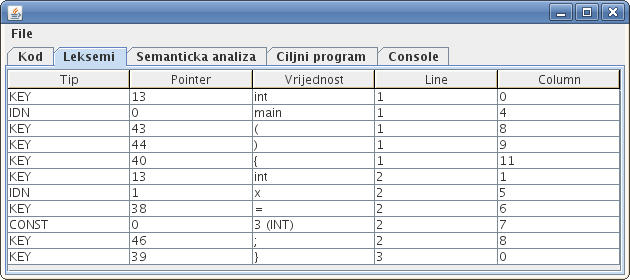
\includegraphics[width=13cm]{primjer-leksicka1}
  \caption{Primjer izvođenja leksičke analize}
\label{komponente}
\end{figure}
